\section{Cape of Good Hope - Postal History 
} 

\begin{figure}[htbp]
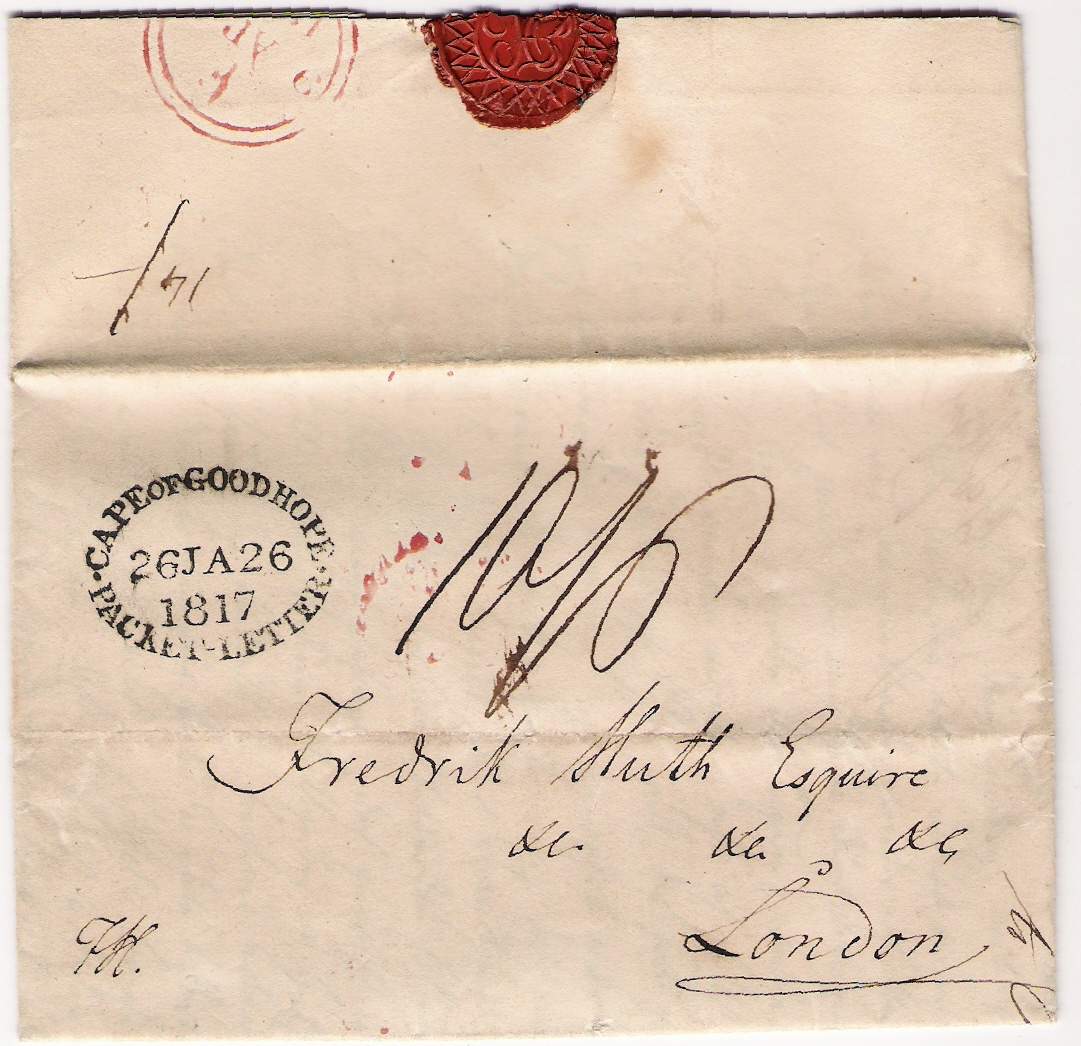
\includegraphics[width=.95\textwidth]{../cape-of-good-hope/Packet/PacketLetter.jpg}
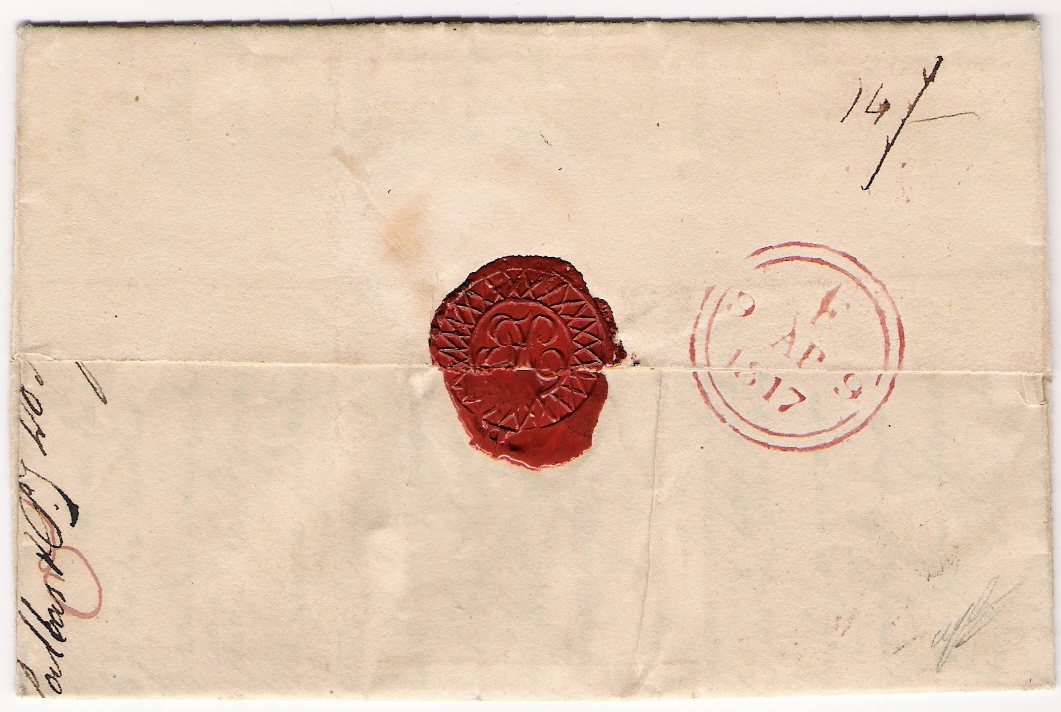
\includegraphics[width=.95\textwidth]{../cape-of-good-hope/Packet/PacketLetterBackstamp.jpg}
\caption{
1817 'Packet Letter' hanstamp entire letter Cape Town to London bearing extremely fine impression of the scarce unlined oval Cape of Good Hope 'Packet Letter' handstamp dated '26 JA 1817' (Goldblatt PL1), arrival backstamp in red '9 AP 17', rated at 10/6 which was three times the basic single letter sheet rate, refolded horizontally
}
\end{figure}

The 'Packet Letter' Datestamp was issued  in 1816 as a result of the 
Ship Letter Act of 1815. While in operation all letters carried by 
packet boats to and from the Cape had to have an official post 
office handstamp. During 1816 a dated Packet Letter stamp (PL 1) 
was issued to the post office at Cape Town. Goldblatt reports 
the earliest known date to be 3 May 1816.

(For a discussion of the Ship Letter Act of 1815 and its effect on 
Cape mail see Palimpsest Letters).

The design of the handstamp was similar to the design of packet 
letter stamps also provided for St. Helena, Mauritius, Calcutta, 
Bombay, Madras and Ceylon. It was oval and unlined. The words 
'Cape of Good Hope' forms the upper section of the oval with 
'Packet Letter' forming the lower. The day month and year are 
in the middle of the oval postmark.

This was the first handstamp in use at the Cape of Good Hope 
which incorporated a date in its design.

This handstamp is considered to be the scarcest of the early 
postal history of the Cape of Good Hope with only about twelve copies recorded.



	 
                                              